\documentclass[11pt,a4paper]{article}
\usepackage{graphicx}
\usepackage{dirtytalk}
\usepackage{acl2021}
\usepackage{natbib}
\bibliographystyle{abbrvnat}
%%\addbibresource{lit.bib}
\usepackage{times}
\usepackage{latexsym}
\renewcommand{\UrlFont}{\ttfamily\small}
\setlength{\textfloatsep}{10pt plus 1.0pt minus 5.0pt}
\vspace{1pt}

% This is not strictly necessary, and may be commented out,
% but it will improve the layout of the manuscript,
% and will typically save some space.
\usepackage{microtype}

%\aclfinalcopy % Uncomment this line for the final submission
%\def\aclpaperid{***} %  Enter the acl Paper ID here

%\setlength\titlebox{5cm}
% You can expand the titlebox if you need extra space
% to show all the authors. Please do not make the titlebox
% smaller than 5cm (the original size); we will check this
% in the camera-ready version and ask you to change it back.

\newcommand\BibTeX{B\textsc{ib}\TeX}

%\aclfinalcopy % Uncomment this line for the final submission
%\def\aclpaperid{***} %  Enter the acl Paper ID here

%\setlength\titlebox{5cm}
% You can expand the titlebox if you need extra space
% to show all the authors. Please do not make the titlebox
% smaller than 5cm (the original size); we will check this
% in the camera-ready version and ask you to change it back.

\title{Changes in Baselines of Hatespeech Detection with pretraining and Transformers}
\author{Matthias Westenfelder}


\begin{document}
\maketitle
\tableofcontents
\begin{abstract}
In this project we aim to construct a new representative baseline for Deep Neural Nets on the HatefulTwitter dataset proposed by \cite{auto_hatespeech}.
For this we implement a Transformer-based Architecture on the data and try to push the baselines proposed by the authors of the HatefulTwitter dataset.
Then we will aim to provide some evaluation of explainability and performance, also with respect to industry usecases.
\end{abstract}
 

\section{Introduction}
In their paper \cite{auto_hatespeech} propose a tweet dataset with 25.000 entries and use some basic methods to establish baselines,
especially interesting is that BoW approaches seem to have major problems distinguishing between hatespeech and offensive language since the distributions are so similar.
This might indicate that context sensitive methods are to be used. For example Transformers/BERT-models yield such a functionality.
As a convention we will use \textbf{bold font} to refer to codebase related entities, for example: 
"...in the notebook \textbf{data\_pipeline} one finds the function \textbf{preprocess\_tweet} which handels preprocessing".

\subsection{The Research Question}

\section{Review of \cite{auto_hatespeech}}
In this section the central question is: "What did Davidson et al. actually do?" and "What are the results against which we will benchmark?".

\subsection{the Model}
The jist oft is the following:
They use a dataset with about 25.000 tweets. 
Then use Tidf-vectorizers on the tokens and on the POS-tags of the tweet to get a vectorized 
version of the tweet on the syntactic and on the word-level.
Then calculate a few more features based on reading-ease levels, counts of hashtags,mentions,urls and sentiment.
All these get fed into a feature selecter via logistic regression with L1-regularization ( using the liblinear solver )
for dimensionality reduction and then predictions are generated using a \textbf{LinearSVC} with L2-penalty and squared hinge loss.

\subsection{the Results}
\cite{auto_hatespeech} claims that their final model has an overall precision of 0.91, an overall recall of 0.9 and a f1-score of 0.9.
They also claim a precision of 0.44 and recall of 0.61 (which implies a F1-score of about 0.525) on the hate class.
These claims come with an asteriks, because these numbers do not represent the performance on a test set but rather using the entire
data to train and evaluating effectively on the trainingset. 
It is impossible to really judge how much overfitting inflates the numbers here, but to keep everything compareable we will use this methodology as well.
What we were able to replicate is a model which achieves overall precision 0.87, recall of 0.85 and F1-score of 0.85 
trained and evaluated on the entire dataset.
And a precision of 0.48, recall of 0.47 and an F1-score of 0.44 on the hateclass.
Which is close to the reported values but still quite a bit less than what was reported.

\begin{table}
\caption{classification report for our reporduction of Davidsons model with features}
\resizebox{\linewidth}{!}{
\begin{tabular}{c| c c c c}
class & precision & recall & f1-score & support \\
\hline
hateful & 0.5 & 0.4 & 0.44 & 1430.0 \\
offensive & 0.95 & 0.87 & 0.91 & 19190.0 \\
neither & 0.63 & 0.91 & 0.75 & 4163.0 \\
\end{tabular}}

\resizebox{\linewidth}{!}{
\begin{tabular}{c| c c c c}
metric & precision & recall & f1-score & support \\
\hline
accuracy & nan & nan & 0.85 & 24783.0 \\
macro & 0.69 & 0.73 & 0.7 & 24783.0 \\
weighted & 0.87 & 0.85 & 0.85 & 24783.0 \\
\end{tabular}}

\label{tab:davidson_withfeat}
\end{table}

Since we aim to compare the embeddings only we reran the sourcecode of Davidson with just the vectorizers on the tweet and the pos-tags.
This yielded a model with overall precision of 0.87, recall of 0.85, F1-score of 0.86
and a precision of 0.4, a recall of 0.53 and a F1-score of 0.46 on the hateclass.

\begin{table}
\caption{classification report for our reporduction of Davidsons model without features} 
\resizebox{\linewidth}{!}{
\begin{tabular}{c| c c c c}
class & precision & recall & f1-score & support \\
\hline
hateful & 0.4 & 0.53 & 0.46 & 1430.0 \\
offensive & 0.94 & 0.88 & 0.91 & 19190.0 \\
neither & 0.69 & 0.84 & 0.76 & 4163.0 \\
\end{tabular}}

\resizebox{\linewidth}{!}{\begin{tabular}{c| c c c c}
metric & precision & recall & f1-score & support \\
\hline
accuracy & nan & nan & 0.85 & 24783.0 \\
macroavg & 0.68 & 0.75 & 0.71 & 24783.0 \\
weightedavg & 0.87 & 0.85 & 0.86 & 24783.0 \\
\end{tabular}}


\label{tab:davidson_nofeat}
\end{table}

The confusion matricies can be seen in \ref{fig:feature_confusion} and \ref{fig:nofeature_confusion}.

\begin{figure}[h]
  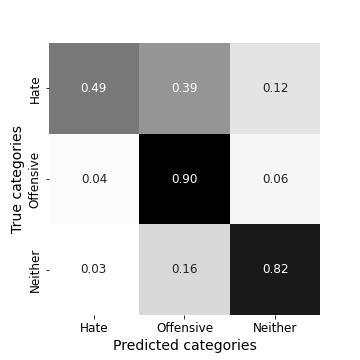
\includegraphics[width=\linewidth]{./tables-figures/feat_confusion.jpg}
  \caption{Confusion of our version of Davidsons model with features}
  \label{fig:feature_confusion}
\end{figure}

\begin{figure}[h]
  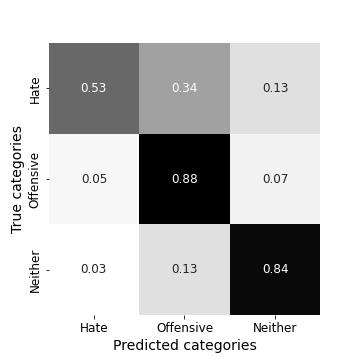
\includegraphics[width=\linewidth]{./tables-figures/nofeat_confusion.jpg}
  \caption{Confusion of our version of Davidsons model with no features}
  \label{fig:nofeature_confusion}
\end{figure}

\section{The Model and Implementation}

\subsection{The preprocessing}
For preprocessing of the Tweets we used the Spacy \textbf{en\_core\_web\_sm} pipeline with \textbf{EntityRuler} Component added.
Which uses identical RegEx to Davidson to identify urls mentions and excess whitespace.
Then the entire tweet is lemmatized via the \textbf{Lemmatizer} component in the \textbf{en\_core\_web\_sm} pipeline and urls 
are replaced with a "[URL]" token, as well as mentions being replaced by a "[MENTION]" token.
The entire procedure is handeled in the function \textbf{preprocess\_tweet} in the \textbf{data\_pipeline} notebook.
Here some possible improvements would be to also have a dedicated "[HASHTAG]" token as well as dealing better with elongated
versions or slightly modified versions of the same tokens. 
For example: turning "Shuuuuuuuuut upppp" or "\$hut up" into "shut up".

\subsection{The Model}
For the model we used a \textbf{distil-bert-uncased} pretrained Distilbert model with a classification head for finetuning
using the Huggingface \textbf{AutoModelForSequenceClassification} class. In addition we used the appropriate BERT-WordPiece 
tokenizer adding two custom tokens ([URL],[MENTION]) to the tokenizer.
The model gets called by the \textbf{Trainer} class via a \textbf{model\_init} method, since otherwise the classification head
weights are not connected to the \textbf{seed} parameter of the \textbf{Trainer} class.
This turns out to be a great problem to get reproducable results.
Especially in our experiments, this turned out to be a problem, since the best model we trained was not able to be replicated,
with the set seed since, we simply got lucky with the classification head weights. Which is exactly why we now use a \textbf{model\_init} method.
And also why it shouldn't be expected to get the exact weights we got once the training procedure is followed.
Which is why the Pytorch model is provided completely in the repository to make the results reproducable.

\subsection{Finetuning}
We used a custom lossfunction to mediate classimbalances.
For this we subclassed the \textbf{Trainer} class and overwrote the \textbf{compute\_loss} function with a custom function.
We use \textbf{CategoricalCrossEntropy} with weights for each class given by:
$$ w_i = 1 - \frac{count(class_i)}{count(data)}$$
For training we used the following Hyperparameters:
First we finetuned with: 
\begin{itemize}
    \setlength{\itemsep}{0.5pt}
    \item learning\_rate = 1e-5
    \item per\_device\_train\_batch\_size = 16
    \item per\_device\_test\_batch\_size = 16
    \item num\_train\_epochs = 5
    \item weight\_decay=0.01
    \item evalution\_strategy = "steps"
    \item eval\_steps = 500
    \item fp16 = True
    \item load\_best\_model\_at\_end = True
    \item metric\_for\_best\_model = eval\_hatef1
    \item seed = 42
\end{itemize}

Then we finetuned another pass with changes only in:

\begin{itemize}
    \setlength{\itemsep}{0.5pt}
    \item learning\_rate = 5e-6
    \item num\_train\_epochs = 2
    \item seed = 42
\end{itemize}
the rest of the unspecified hyperparameters were the default value or are paths/logging settings which aren't training
relevant and can be looked up in the \textbf{train\_model} notebook.

\subsection{Results}
This yielded the following results using sklearns \textbf{classification\_report}.
\begin{table}
\caption{Classification report for our finetuned model without external features}
\resizebox{\linewidth}{!}{
\begin{tabular}{c| c c c c}
class & precision & recall & f1-score & support \\
\hline
hateful & 0.56 & 0.71 & 0.63 & 1430.0 \\
offensive & 0.97 & 0.95 & 0.96 & 19190.0 \\
neither & 0.94 & 0.97 & 0.95 & 4163.0 \\
\end{tabular}}

\resizebox{\linewidth}{!}{
\begin{tabular}{c| c c c c}
metric & precision & recall & f1-score & support \\
\hline
accuracy & nan & nan & 0.94 & 24783.0 \\
macroavg & 0.83 & 0.88 & 0.85 & 24783.0 \\
weightedavg & 0.94 & 0.94 & 0.94 & 24783.0 \\
\end{tabular}}

\label{tab:model}
\end{table}

\ref{tab:model} shows that one can expect a relatively basic transformer model to outperform the baseline proposed by \cite{auto_hatespeech}.
The most significant improvement on the hateclass, that is pretty stable, under multiple training runs (different seeds and random classifier head weights)
is the precision. It is not uncommon to see with finetuning for a few epochs a precision of 0.5 and a recall of 0.5 on the hateclass of the testset.
This still is a 0.06 improvement in precision over Davidsons reported numbers.
Here one starts to see a form of Precision/Recall Trade-off emerge when training where one needs some trial and error to get a model for which 
$$ Recall + Precision > 1 $$

\begin{figure}[h]
 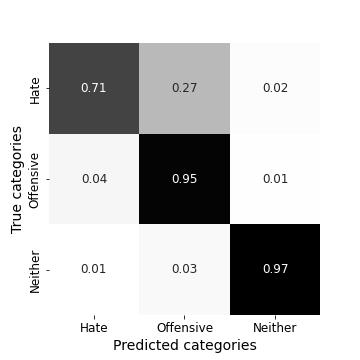
\includegraphics[width=\linewidth]{./tables-figures/model_confusion.jpg}
  \caption{Confusion of the finetuned model}
  \label{fig:model_confusion}
\end{figure}

\section{Evaluation}
\subsection{Comparison to \cite{auto_hatespeech}}
Comparing \ref{tab:model} to the reported numbers in Davidsons paper we can clearly see the overall performance increase
\begin{table}[h]
  \begin{tabular}{c | c  c}
    metric & our model & Davidson \\
    \hline
    precision-avg &  0.95 & 0.91 \\
    recall-avg &  0.94 & 0.90 \\  
    f1-score-avg &  0.95 & 0.9 \\
  \end{tabular}
\end{table}

Especially interesting is the improvement on the hate-class of the transformer model, especially with tuned Hyperparameters and
finding good initial weights in the classification head the finetuned transformer model outperforms the Baseline by Davidson reliably.

\begin{table}[h]
  \begin{tabular}{c | c  c}
    metric & our model & Davidson \\
    \hline
    hate-precision &  0.58 & 0.44 \\
    hate-recall &  0.75 & 0.61 \\  
    hate-f1-score &  0.66 & 0.53 \\
  \end{tabular}
\end{table}

\subsection{Confusion and Maximum loss}
We first begin to investigate some confusions of the model, for this purpose we use the \textbf{get\_top\_loss} function and investigate the examples which
caused the biggest contributions to the loss.
A typical error of the model is to overfit on the frequency of slurrs like "bitch","hoe" and similar.
These get classified almost universally as offensive independend of the context they were used.
A few examples of a tweets which were classified as offensive but are actually part of the neither class would be

\paragraph{Examples of confusing neither with offensive class:}
\begin{center}
  \say{I don't know what you been told but I love them project hoes} \newline
  \say{No girls no hoes just me myself and I} \newline
  \say{Up early then a bitch driving to denton omg can I move already} \newline
  \say{Frustration can be a bitch !}\newline
\end{center}

Especially interesting is this example which illustrates the overfitting quite well:

\begin{center}
 \say{School Schoo Scho Sch Sc S St Sta Stay Stay h Stay ho Stay hom Stay home}
\end{center}

in this tweet the subword "ho" is so close to "hoe" that the model immediately thinks the tweet is offensive.
This can be seen in the attention patterns of the model as seen in \ref{fig:school-saliency}

The same overfitting on some special token frequency also leads to confusion between the hateful and offensive class.
While confusion between the neither and hateful class occurs often in two types.
The first type of error the model makes is not recognizing directed offensiveness versus undirected offensiveness.
While the second type of error the model makes, is not seeing masked offensiveness.
Where user use slurrs that don't have a high enough frequency tobe recognized as such 
or where everyday objects get used creatively to create offensive context.

\paragraph{Examples of confusions in the hateful-class}
The tweets below were classified as belonging to the neither-class but belong to the hateful-class.

\begin{center}
 \say{Twice divorced teabagger Florida Attorney General says marriage is reserved for 'stable, enduring family units' http://t.co/9ZWr3O33iu \#wtf} \newline
 \say{@Flow935 jus wanted to let y\&\#225;ll know hope the hurricane kills your soca sunday trash \#LORDWILLIN} \newline
\end{center}

Both don't feature obvious offensive words and really become hateful by directing offensiveness towards someone personally, 
these are good examples of the first type of error.
While these Tweets, which also belong to the hateful-class and were classified as part of the neither-class, showcase the second type of error.
\begin{center}
  \say{stuffed her like an Oreo http://t.co/mPAjkWJbZp}\newline
  \say{Porch monkey 4 Life} \newline
  \say{You are a jiggaboo...!} \newline
\end{center}

The first type of error also tends to mix with the overfitting on sexists-slurrs as seen in the following tweets which were classified as offensive
but which belong to the hateful-class since they direct their offensiveness towards someone.
\begin{center}
  \say{ @Fit4LifeMike @chanelisabeth hoe don't make me put up screenshots of your texts to me hoe }\newline
  \say{@GlitteredInPink hoe don't tweet me}\newline
  \say{RT @Slanguage: Stop flattering yourself, bitch. The only fan you have is on your ceiling.}\newline
\end{center}

Every one of these is a use of "hoe" or "bitch" directed at someone.
These types of errors make up a big portion of the 100 examples with the highest loss in the entire dataset.

\subsection{What did the model learn?}
The investigation of errors yields also some evidence of the model actually learning, instead of only fitting some
frequency correlations. 
This evidence is seen in some of the maximum loss examples, which are just plain misslabled, but get labled correctly by the model.

\paragraph{Examples of tweets that belong in the neither-class:}
\begin{center}
\say{Bae made me deep fried Oreos \&\#128523;}\newline
\say{@VinceSchilling Vince, what is the general feeling of the natives that you know in regards to the term "redskins"? Offensive to them or not?}\newline
\say{wishing I could high five whoever named a species of birds "great tits"}\newline
\say{RT @BALTsneakerShow: Water is wet. RT @202SOLE: Nike DC is trash.}\newline
\say{Chocolate cake is so trash.}\newline
\end{center}

\paragraph{Examples of tweets that belong in the offensive-class:}
\begin{center}
\say{You wanna find hoes on here? Just follow the chicks who reply with heart eyes under sex gifs}\newline
\say{@vh1ADENECA @260chocolate @4Sunshinejones1 aye, I respect ya hustle and all but dont tweet me anymore trash ass videos...thank u kindly}\newline
\end{center}

\paragraph{Examples of tweets that belong in the hateful-class:}
\begin{center}
\say{Looks like a tool but is useful as a clay hammer \#fag @hOPPondis http://t.co/K7wqlAWRwM}\newline
\end{center}

This is not yet complete evidence, but already provides some confidence that the model actually learned some reasonable structure from the ground up.
The model definitely learned about rasist remarks a few of the highest confidence examples in the hate-class revolve around homophobic or racist language.
As one can see in the saliencey scores using the \textbf{multiclass\_explainer} in the \textbf{evaluate\_model} notebook.
example outputs with high confidence are shown in \ref{fig:racism-example},
as one can see in these examples the model derives almost all confidence out of racist-slurrs.



\subsection{Cost of Implementation and viability for industry purposes}

\section{Conclusion - A Reasonable Baseline for Hatespeech}
So we are now able to confidently answer our research question.
Yes we should put forward a different Baseline performance for Transformer models on this dataset.
We propose a good conservative baseline be a recall of 0.65 and precision of 0.55 on the hate-class
with just embeddings, without external features and at least an F1-Score of 0.93 overall.
This is a reasonable perfomance to expect of a Transformer model with a Sequential-head with finetuning
and hyperparameter tuning.
We didn't implement a real Hyperparameter optimization and on a faster GPU, it is possible to get a much deeper search into
the parameter space. Thus this seems like an appropriate baseline, especially wih the results of davidson, being only partially reproducable.




\clearpage 
\appendix

\section{Figures}
\begin{figure}[!ht]
  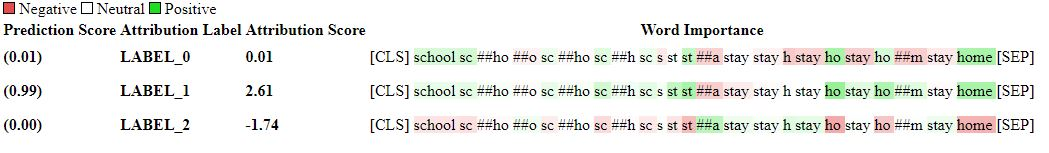
\includegraphics[width=2\linewidth]{./tables-figures/school-confusion-viz.JPG} 
  \caption{saliencey scores for the "school stay home" example}
  \label{fig:school-saliency}
\end{figure}

\begin{figure}[!ht]
  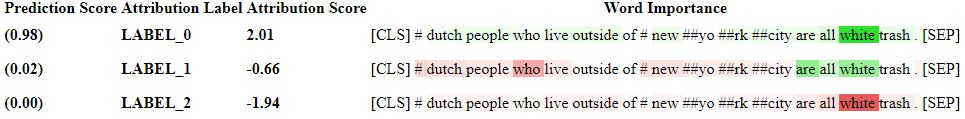
\includegraphics[width=2\linewidth]{./tables-figures/white-trash-example.JPG} 
  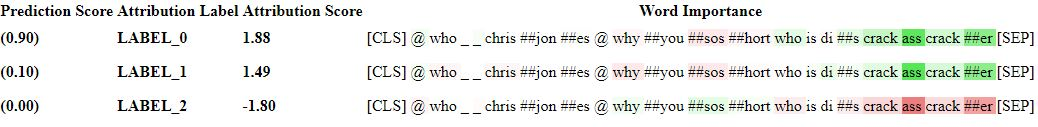
\includegraphics[width=2\linewidth]{./tables-figures/racism-example.JPG} 
  \caption{The model gets strong signal from racist remarks}
  \label{fig:racism-example}
\end{figure}
\bibliography{lit}

\end{document}
